\documentclass[12pt, UTF8]{article}
\usepackage[a4paper, scale = 0.8]{geometry}
\usepackage{ctex}

\usepackage{enumitem}
\usepackage{listings}
\usepackage{xcolor}
\usepackage{color}
\definecolor{GrayCodeBlock}{RGB}{241, 241, 241}
%\definecolor{BlackText}{RGB}{110, 107, 94}
\definecolor{BlackText}{RGB}{0, 0, 0}
\definecolor{RedTypename}{RGB}{182, 86, 17}
\definecolor{GreenString}{RGB}{96, 172, 57}
\definecolor{PurpleKeyword}{RGB}{184, 84, 212}
\definecolor{GrayComment}{RGB}{170, 170, 170}
\definecolor{GoldDocumentation}{RGB}{180, 165, 45}
\lstset {
  columns = fullflexible, keepspaces = true, showstringspaces=false, breaklines = true, frame = single, framesep = 0pt, framerule = 0pt, framexleftmargin = 4pt, framexrightmargin = 4pt, framextopmargin = 5pt, framexbottommargin = 3pt, xleftmargin = 4pt, xrightmargin = 4pt,
  backgroundcolor = \color{GrayCodeBlock},
  basicstyle = \ttfamily\color{BlackText},
  keywordstyle = \color{PurpleKeyword},
  ndkeywordstyle = \color{RedTypename},
  stringstyle = \color{GreenString},
  commentstyle = \color{GrayComment}
}

\usepackage{graphicx}
\usepackage{amsmath}

\usepackage[colorlinks, linkcolor = red, anchorcolor = blue, citecolor = green]{hyperref}

\usepackage{soul}
\newcommand{\ctext}[1]{
  \begingroup
  \sethlcolor{GrayCodeBlock}
  \hl{#1}
  \endgroup
}
\soulregister{\ttfamily}{1}
\newcommand{\inline}[1]{\ctext{\ttfamily{#1}}}

\renewcommand\thesection{\arabic{section}}

\title{嵌入式系统实验报告}
\author{李晨昊 2017011466}
\begin{document}
\maketitle
\tableofcontents

\section{概述}

我采用简单的模板匹配方法来识别图像位置,基于OpenCV实现。程序自己负责录制视频,在8080端口上应答视频流,在8081端口上应答识别坐标。

最终生成的压缩的镜像文件大小为8.1MiB。以下所有内容都是描述得到这个镜像文件的大致过程,难免有不精确的地方,想要复现这个过程请参考git仓库\href{https://github.com/MashPlant/rpi-image-locating}{rpi-image-locating}。

\section{实现思路}

程序中共运行四个线程,任务分别如下:

\begin{itemize}
  \item \inline{video\_server\_fn}:监听8080端口,运行HTTP服务器,应答视频流。
  \item \inline{pos\_server\_fn}:监听8081端口,运行HTTP服务器,应答识别坐标及接受请求,更换被匹配的图片。
  \item \inline{calc\_fn}:计算识别坐标。
  \item 主线程:录制视频,获取图像。
\end{itemize}

其实\inline{pos\_server\_fn}的工作也可以拆成两个线程完成,不过这样写更简洁一些。而且考虑到Raspberry Pi 3的Cortex-A53刚好四颗核心,也许运行四个线程比较合适。

\subsection{识别方法}

需要确定摄像头中的图片在完整图片中占多少像素,我是通过让屏幕显示一张标满刻度的图片,数刻度计算得到的,在我的环境中是\inline{VIDEO\_W = 234, VIDEO\_H = 156}。

将摄像头拍摄的图片resize到这个大小,然后和待匹配图片做同样次数的\inline{pyrDown}操作。我选择压缩三次,因为压缩两次时识别帧率只能达到十几,而压缩三次时帧率达到了30,这也是图像录制的帧率,计算更快也没有意义了,就选择三次。

压缩后调用\inline{matchTemplate}函数,我使用的方法是\inline{TM\_CCORR\_NORMED},没有使用mask矩阵。直接把匹配矩阵的最大值的位置作为识别的位置发给电脑端,电脑端负责根据这个坐标在图片上绘制白框标明识别位置。

\subsection{实现简单的HTTP服务器}

网络上有一些C++的HTTP开源实现,但是最简单的也以千行记,而且很多都不支持我需要的功能(发送视频流)。我手动了实现一个虽然非常不规范,但是也能满足需求且足够简单的HTTP服务器。所谓的HTTP协议也就是TCP socket上的请求和响应遵守一定的文字格式,只要我手动把这些文字写入socket就行了。

8080端口上不需要接受客户端的任何信息,对任何请求都回复视频流,所以不需要从socket中读任何内容。回复视频流的格式是参照助教的Python示例编写的,先发送一个回复:

\begin{lstlisting}
HTTP/1.1 200 OK\r\n
Content-Type: multipart/x-mixed-replace; boundary=--jpg\r\n
\r\n
\end{lstlisting}

然后循环发送以下内容:

\begin{lstlisting}
--jpgHTTP/1.1 200 OK\r\n
Content-Type: image/jpeg\r\n
Content-length: <编码的图片的长度>\r\n
\r\n
<编码的图片的数据>
\end{lstlisting}

因为是简单地向一个socket循环发送,所以同一时间只能服务一个客户端,这在我的应用中也足够了。

8081端口可以处理两种请求,一种是GET,回复识别出的坐标;一种是POST,按照客户端的要求更换被匹配的图片。目标图片的编号在客户端用query string传递:

\begin{lstlisting}[language=c]
fetch(server + "8081?pic=" + pic, { method: "POST" })
\end{lstlisting}

此时可以在socket中读到一段HTTP请求,开头内容是\inline{POST /?pic=x},所以在我的实现中如果第11个字符是\inline{=}就认为是POST请求,然后根据第12个字符的内容更换图片。

在我开发了这个功能后才知道不需要在运行时更换被匹配的图片,所以程序中只实现了读出这个字符,没有进行实际的更换图片操作。

\section{构建应用程序}

我使用musl工具链交叉编译生成静态可执行程序,这样的好处在于不需要为了这个程序安装任何依赖,后面构建系统的时候更简单。

\subsection{编译OpenCV}

OpenCV仓库中\inline{platforms/linux/}下定义了很多CMake Toolchain文件,其中没有musl工具链的,但是\inline{arm-gnueabi.toolchain.cmake}比较接近我们的需求,可以基于它修改出一份\inline{arm-musleabi.toolchain.cmake},只需要把\inline{GNU\_MACHINE "arm-linux-gnueabi"}修改成\inline{GNU\_MACHINE "arm-linux-musleabi"}即可,注意\inline{GNU\_MACHINE}这个名字不能修改,因为后续会用到。

用以下指令编译:

\begin{lstlisting}[language=bash]
$ git clone https://github.com/opencv/opencv && cd opencv
$ mkdir build_musl && cd build_musl
$ cmake -DCMAKE_TOOLCHAIN_FILE=../platforms/linux/arm-musleabi.toolchain.cmake -DBUILD_SHARED_LIBS=OFF -DCMAKE_BUILD_TYPE=Release -DCMAKE_INSTALL_PREFIX=../install_musl ..
\end{lstlisting}

因为我的目标是最终编译一个静态链接的程序,编译出的OpenCV也需要是静态的,所以指定\inline{BUILD\_SHARED\_LIBS=OFF}。OpenCV的CMake文件写的比较完善,在识别出是交叉编译的情况下会自动从源码编译需要的依赖和关闭一些额外的支持,所以不需要什么额外的配置。

\inline{cmake}可能会报错说没法编译测试程序,因为\inline{arm-linux-gnueabihf-gcc}目前不支持Thumb模式下的Hard Float API。在\inline{arm.toolchain.cmake}中找到了两个\inline{-mthumb}选项,把它们去掉即可:

\begin{lstlisting}[language = c, ndkeywords = {set, STREQUAL}, escapeinside={(*@}{@*)}]
if(CMAKE_SYSTEM_PROCESSOR STREQUAL arm)
  set(CMAKE_CXX_FLAGS "(*@\color{GreenString}{\st{-mthumb}}@*) ${CMAKE_CXX_FLAGS}")
  set(CMAKE_C_FLAGS "(*@\color{GreenString}{\st{-mthumb}}@*) ${CMAKE_C_FLAGS}")
  set(CMAKE_EXE_LINKER_FLAGS "${CMAKE_EXE_LINKER_FLAGS} -Wl,-z,nocopyreloc")
endif() 
\end{lstlisting}

重新\inline{cmake}后执行\inline{make install -j16},把OpenCV的库文件和头文件安装到\inline{<opencv path>/install}下。\inline{make install}是有必要的,我之前按照平时的习惯直接\inline{make}后\inline{build}文件夹下已经有了库文件,并且我之前在本机安装过OpenCV,所以系统include路径中也有必要的头文件,但是这两个配合在一起使用时,编译程序的时候出现了找不到符号的链接错误。具体原因我不确定,可能与头文件中定义的调用约定有关,也可能是\inline{build}下的库文件自身的问题。

\subsection{编译程序}

写一个简单的测试程序:

\begin{lstlisting}[language=c++]
#include <opencv2/core.hpp>
#include <opencv2/imgcodecs.hpp>
#include <opencv2/videoio.hpp>

int main() {
  cv::VideoCapture video(0);
  cv::Mat pic;
  if (video.read(pic)) {
    imwrite("a.jpg", pic);
  }
}
\end{lstlisting}

编译参数:

\begin{lstlisting}[language=bash]
$ arm-linux-musleabihf-g++ main.cpp -I<opencv path>/install_musl/include/opencv4/ -L<opencv path>/install_musl/lib -lopencv_stitching -lopencv_video -lopencv_calib3d -lopencv_features2d -lopencv_flann -lopencv_objdetect -lopencv_ml -lopencv_highgui -lopencv_videoio -lopencv_imgcodecs -lopencv_photo -lopencv_imgproc -lopencv_core -L<opencv path>/install_musl/lib/opencv4/3rdparty -littnotify -llibjpeg-turbo -llibopenjp2 -llibpng -llibprotobuf -llibtiff -llibwebp -lquirc -lzlib -ldl -lpthread -O3 -static
\end{lstlisting}

这些\inline{-lopencv\_...}的顺序很重要,因为是静态链接,所以每个库文件必须出现在依赖它的库文件之后。我没有什么好方法得到这个顺序,是通过运行本机上的\inline{pkg-config --libs opencv},然后去掉其中不存在的库得到的。后面\inline{-l}第三方库的顺序应该无所谓,因为它们之间没有什么依赖关系。

\subsection{修复运行错误}

上一步生成了一个ARM的静态可执行程序,可以把它拷贝到树莓派上运行,但是只得到了一些警告信息,没有生成图片:

\begin{lstlisting}[language=bash]
$ ./a.out
[WARN:0] ... videoio/src/cap_v4l.cpp (823) createBuffers VIDEOIO(V4L2:/dev/video0): failed VIDIOC_QUERYBUF: errno=25 (Not a tty)
[WARN:0] ... videoio/src/cap_v4l.cpp (893) open VIDEOIO(V4L2:/dev/video0): can't open camera by index
\end{lstlisting}

看起来是一次\inline{ioctl}调用失败了,下面是我尝试解决这个问题的过程。最终得到的解决方案是更换老版本的musl工具链(1.1.24或以下)。

我用\inline{arm-gnueabi.toolchain.cmake}重新编译了OpenCV和测试程序(只能生成动态链接的程序),这样得到的程序是可以运行的。设置OpenCV的log等级为\inline{LOG\_LEVEL\_DEBUG},对比二者的log,关键的一行在于:

\begin{lstlisting}[escapeinside={(*@}{@*)}]
gnu : [DEBUG:0] ... videoio/src/cap_v4l.cpp (967) tryIoctl VIDEOIO(V4L2:/dev/video0): call ioctl(3, VIDIOC_QUERYBUF((*@\color{red}{3226490377}@*)), ...) => -1    errno=25 (Not a tty)
musl: [DEBUG:0] ... videoio/src/cap_v4l.cpp (967) tryIoctl VIDEOIO(V4L2:/dev/video0): call ioctl(3, VIDIOC_QUERYBUF((*@\color{red}{3225703945}@*)), ...) => 0    errno=0 (No error information)
\end{lstlisting}

\inline{VIDIOC\_QUERYBUF}是一个宏,它作为第二个参数传入\inline{ioctl}系统调用,但是在这两个程序中它的值不一样。两个编译器下它的定义都是:

\begin{lstlisting}[language=c++]
#define VIDIOC_QUERYBUF		_IOWR('V',  9, struct v4l2_buffer)
\end{lstlisting}

但是两个编译器下\inline{struct v4l2\_buffer}的大小不一样,\inline{arm-linux-gnueabihf-gcc}下是68,\inline{arm-linux-musleabihf-gcc}下是80,进一步原因在于其中的\inline{struct timeval}的大小不一样,分别为8和16,再加上内存对齐,就差了12字节。

查到\href{https://musl.libc.org/time64.html}{musl time64 Release Notes}中对此有解释,从版本1.2.0开始\inline{time\_t}大小从32位变为64位。其中也提到了\inline{ioctl}的问题,但它声称musl库中包含了处理这种不兼容性的代码。\href{https://github.com/ifduyue/musl/blob/d91a6cf6e369a79587c5665fce9635e5634ca201/src/misc/ioctl.c#L51}{src/misc/ioctl.c:51}确实提到了\inline{VIDIOC\_QUERYBUF}:

\begin{lstlisting}[language=c]
/* VIDIOC_QUERYBUF, VIDIOC_QBUF, VIDIOC_DQBUF, VIDIOC_PREPARE_BUF */
{ _IOWR('V',  9, new_misaligned(72)), _IOWR('V',  9, char[72]), 72, WR, 0, OFFS(20) },
{ _IOWR('V', 15, new_misaligned(72)), _IOWR('V', 15, char[72]), 72, WR, 0, OFFS(20) },
...
\end{lstlisting}

但是它的实现似乎有点问题,它认为\inline{struct v4l2\_buffer}在老版本中的大小是72,但实际是68,这导致生成的数值匹配不上,那它就不会做这个翻译转化的工作。

我把新版本的musl中这里的72改成68,用\href{https://github.com/richfelker/musl-cross-make}{musl-cross-make}编译musl工具链,再用编译出的工具链重复之前的工作,结果是这个ioctl调用确实成功了,但是后续的一次\inline{mmap}调用还是失败了,我目前还没有找出原因,只能放弃这个方向了。

我又尝试了1.1.24版本的musl工具链,这时\inline{time\_t}还是32位的。重复之前的工作,最终程序能够正常运行了。得到老版本的musl工具链也是通过\href{https://github.com/richfelker/musl-cross-make}{musl-cross-make},修改\inline{Makefile}中的版本号即可。

\subsection{裁剪程序}

最初编译好的程序大小达到15.2MiB,这里记录了我优化程序尺寸的过程。

\begin{enumerate}
  \item 去除符号信息。不需要手动调用\inline{arm-linux-musleabihf-strip},在\inline{arm-linux-musleabihf-g++}编译时加一个\inline{-s}参数即可。尺寸从15.2MiB降到5.9MiB。
  \item 去掉我不需要的图像格式。OpenCV的\inline{imgcodecs}模块中支持很多图像格式,包括PNG,WEBP等,但是我的应用中只需要用到JPEG格式,所以通过cmake选项去掉这些格式的支持。OpenCV顶层的\inline{CMakeLists.txt}中定义了很多选项,可以手动传入值关掉,但是这些图像相关的选项并没有放在一起,也没有统一的文档介绍,我是通过\href{https://github.com/opencv/opencv/blob/master/modules/imgcodecs/src/loadsave.cpp#L137}{modules/imgcodecs/src/loadsave.cpp:137}开始的一系列宏找到它们的。添加cmake参数:

\begin{lstlisting}
-DWITH_PROTOBUF=OFF -DWITH_IMGCODEC_HDR=OFF -DWITH_WEBP=OFF -DWITH_IMGCODEC_SUNRASTER=OFF  -DWITH_IMGCODEC_PXM=OFF -DWITH_IMGCODEC_PFM=OFF -DWITH_TIFF=OFF -DWITH_PNG=OFF -DWITH_GDCM=OFF -DWITH_JASPER=OFF -DWITH_OPENJPEG=OFF -DWITH_OPENEXR=OFF -DWITH_GDAL=OFF
\end{lstlisting}

  尺寸从5.9MiB降到5.0MiB。
  
  \item 关闭异常和RTTI支持。众所周知异常和RTTI是C++代码尺寸膨胀的重要原因之一,如果能在OpenCV中关掉异常和RTTI的支持,应该可以减少一定尺寸。直接在编译程序时传入\inline{-fno-exceptions -fno-rtti}是没有任何作用的,因为OpenCV的库代码已经在开启异常和RTTI的情况下编译好了,必须在编译OpenCV时就关掉。
  
  再次修改\inline{arm.toolchain.cmake},添加如下编译选项:

\begin{lstlisting}[language = c, ndkeywords = {set, STREQUAL}, escapeinside={(*@}{@*)}]
if(CMAKE_SYSTEM_PROCESSOR STREQUAL arm)
  set(CMAKE_CXX_FLAGS "(*@\color{red}{-fno-exceptions}@*) (*@\color{red}{-fno-rtti}@*) ${CMAKE_CXX_FLAGS}")
  set(CMAKE_C_FLAGS "(*@\color{red}{-fno-exceptions}@*) ${CMAKE_C_FLAGS}")
  set(CMAKE_EXE_LINKER_FLAGS "${CMAKE_EXE_LINKER_FLAGS} -Wl,-z,nocopyreloc")
endif()
\end{lstlisting}
  
  然后会报出很多编译错误,这是因为OpenCV本身大量使用异常,也少量使用RTTI,关闭它们下就不能正常编译。有一些实际没有用到的模块也报了错,比如\inline{flann},为了减少后面修改代码的工作量,先去掉这些模块。我的应用中只用到\inline{videoio},\inline{imgcodecs},\inline{imgproc},\inline{core}这四个,除此之外全部不编译,添加cmake参数:

\begin{lstlisting}
-DBUILD_opencv_apps=OFF -DBUILD_opencv_calib3d=OFF -DBUILD_opencv_features2d=OFF -DBUILD_opencv_flann=OFF -DBUILD_opencv_gapi=OFF -DBUILD_opencv_highgui=OFF -DBUILD_opencv_java_bindings_generator=OFF -DBUILD_opencv_js=OFF -DBUILD_opencv_ml=OFF -DBUILD_opencv_objdetect=OFF -DBUILD_opencv_photo=OFF -DBUILD_opencv_python_bindings_generator=OFF -DBUILD_opencv_python_tests=OFF -DBUILD_opencv_stitching=OFF -DBUILD_opencv_ts=OFF -DBUILD_opencv_video=OFF
\end{lstlisting}  
  
  注意仅仅不编译它们不会对减小尺寸有任何帮助,因为这些库本来就没有链接到我的程序中。
  
  然后修改代码,去掉\inline{try},去掉\inline{catch}分支,将\inline{throw}异常改成\inline{abort()}。如果有些包含这些关键字的函数我确定不会用到,我就把它整个去掉,这样还更简单一些。粗略统计我用到的四个模块中需要修改50处左右,涉及24个文件。因为我可以确定实际运行时不会发生异常,所以这些改变都不会影响程序运行效果。我还添加了两个cmake参数:\inline{-DWITH\_OPENCL=OFF -DWITH\_PTHREADS\_PF=OFF},相关的代码涉及一些异常处理,而且我应该也用不到这些功能,所以直接关闭这两个选项更方便。
  
  RTTI的使用只有几处,一处是输出log时用来输出类型名称,可以直接去掉;一处是用\inline{dynamic\_cast}来downcast指针,这个本来是不好去掉的,但是它downcast之后紧接着就assert结果非空,因为可以假定assert不会失败,所以可以直接用\inline{static\_cast}代替。
  
  尺寸从5.0MiB降到3.2MiB。
  
  \item 关闭OpenCV的log输出。虽然这些log在我调试的初期给了我巨大的帮助,但是调试完成后就不再需要它们了。修改\inline{modules/core/include/opencv2/core/utils/logger.hpp}中的\inline{CV\_LOG\_WITH\_TAG}宏,直接改成一个空操作。尺寸从3.2MiB降到3.1MiB。
  \item 在OpenCV中固定我调用的函数的参数。OpenCV中很多函数都支持一个“方法”参数,根据它执行不同的算法,这些算法的代码都会保留在最终的二进制程序中,但实际上我只会用到其中的一个,这就浪费了很多空间。理想情况下这种优化可以通过LTO自动完成,但是我编译OpenCV时传入\inline{-flto}参数时报错说缺少插件,可能是编译器还不支持,所以还是需要我手工优化。我固定的参数包括:
  
  \begin{itemize}
    \item \inline{resize}的\inline{interpolation}参数一定是\inline{INTER\_LINEAR}。尺寸从3.1MiB降到3.0MiB。
    \item \inline{cvtColor}的\inline{code}参数一定是\inline{COLOR\_BGR2GRAY}。尺寸从3.0MiB降到2.9MiB。
    \item \inline{matchTemplate}的\inline{method}参数一定是\inline{TM\_CCORR\_NORMED},\inline{mask}一定是空矩阵。尺寸从2.9MiB降到2.4MiB。
  \end{itemize}
  
  \item 此时程序虽然只有2.4MiB,但还依赖一个2.0MiB左右的图片。我的程序只需要图片的灰阶数据,而且用\inline{pyrDown}压缩三次,一张\inline{1920 * 1080}的图片实际用到的信息量只有\inline{(1920 / 8) * (1080 / 8) = 32400B},远小于2.0MiB,所以可以设法把图片数据嵌入到程序中。
  
  借助\href{https://github.com/MashPlant/rpi-image-locating/blob/master/gen_data.cpp}{gen\_data.cpp}输出\inline{cv::Mat}的相关信息:
  
  \begin{lstlisting}[language=c++]
#include <opencv2/core.hpp>
#include <opencv2/imgcodecs.hpp>
#include <opencv2/imgproc.hpp>

int main() {
  cv::Mat p = cv::imread("./1.jpg", cv::IMREAD_GRAYSCALE);
  for (int i = 0; i < 3; ++i) cv::pyrDown(p, p);
  // 输出元信息
  printf("%x %d %d %d\n", p.flags, p.dims, p.rows, p.cols); // 输出 42ff4000 2 135 240
  printf("%p %p %p %p\n", p.data, p.datastart, p.dataend, p.datalimit); // 观察到 data = datastart, dataend = datalimit = data + 240 * 135
  printf("%d %d %ld %ld\n", p.size[0], p.size[1], p.step[0], p.step[1]); // 输出 135 240 240 1
  // 输出数据
  printf("unsigned char data[%d] = {", p.rows * p.cols); // 把这个数组定义拷贝到一个单独的data.cpp文件中一起编译
  for (int i = 0; i < p.rows * p.cols; ++i) {
    printf("%u, ", p.data[i]);
  }
  printf("};");
}
\end{lstlisting}
  
  依据这些信息构建\inline{cv::Mat}:
  
\begin{lstlisting}[language=c++]
const int W = 1920 / (1 << PYR_CNT), H = 1080 / (1 << PYR_CNT);
extern unsigned char data[W * H];
static int size[2] = {H, W};
static size_t step[2] = {W, 1};
p.flags = 0x42ff4000, p.dims = 2, p.rows = H, p.cols = W;
p.datastart = p.data = data, p.dataend = p.datalimit = data + W * H;
p.size.p = size, p.step.p = step;
\end{lstlisting}
  
  程序尺寸从2.4MiB上升到2.5MiB,但是不再需要图片,总体尺寸从4.4MiB降低到2.5MiB。
\end{enumerate}

\section{构建Linux系统}

我使用Buildroot构建Linux系统。我的应用程序是静态编译的,所以不需要为了它在Buildroot中添加任何依赖,在系统启动后并联网后可以直接启动我的程序。

在Buildroot文件夹下执行\inline{make raspberrypi3\_defconfig}生成树莓派的默认配置,然后进行如下配置和裁剪。

\subsection{连接Wi-Fi}

我使用\inline{eudev}管理设备,所以需要前两步。连接Wi-Fi这一步手动检测设备并加载内核模块也是可以的,参考\href{https://unix.stackexchange.com/questions/396151/buildroot-zero-w-wireless}{buildroot-zero-w-wireless},但是我在使用这个方式时不知道后续怎么开启摄像头,而\inline{eudev}自动管理了摄像头,可以直接使用。

\begin{enumerate}
  \item 开启\inline{BR2\_TOOLCHAIN\_BUILDROOT\_WCHAR}:Toolchain -> Enable WCHAR support
  
  默认的libc是uClibc,这个选项是关闭的。如果选择glibc,这个选项是强制开启的。
  
  如果在关闭这个选项的情况下\inline{make},后续再开启它再\inline{make}时可能会发生编译错误,需要完全重新构建,所以推荐一开始就设置好。
  
  \item 开启\inline{BR2\_ROOTFS\_DEVICE\_CREATION\_DYNAMIC\_EUDEV}:System configuration -> /dev management -> Dynamic using devtmpfs + eudev
  
  这个选项依赖于第一步的选项。
  
  \item 开启\inline{BR2\_PACKAGE\_RPI\_WIFI\_FIRMWARE}:Target packages -> Hardware handling -> Firmware -> rpi-wifi-firmware
  
  \item 开启\inline{BR2\_PACKAGE\_IW}:Target packages -> Networking applications -> iw
  
  \inline{iw}是用来连接Wi-Fi的,连接后还需要DHCP工具获取IP地址,我使用\inline{udhcpc},它是BusyBox中的一个应用,已经默认自带了。
  
  \item 新建文件夹\inline{rootfs\_overlay},设定\inline{BR2\_ROOTFS\_OVERLAY}为这个文件夹的位置。在其中创建\inline{rootfs\_overlay/etc/init.d/S60wifi},内容为:
  
  \begin{lstlisting}[language=bash]
  ifconfig wlan0 up
  sleep 1
  iw dev wlan0 connect "test"
  udhcpc -i wlan0
  # 这里可以直接执行程序:/root/a.out
  \end{lstlisting}
  
  rootfs overlay功能会将这个文件夹下的内容加入根文件系统中。原本的文件系统中的\inline{init.d/}中的\inline{rcS}会枚举这个文件夹下\inline{S}开头的文件并按顺序执行,所以创建一个这样的文件即可自动执行,\inline{60}应该可以保证它排在现存的文件之后。\inline{test}是我的手机热点的Wi-Fi名称。经实验\inline{ifconfig wlan0 up}开启\inline{wlan0}后需要等待一段时间再连接Wi-Fi和获取IP地址,否则获取IP地址时会收不到响应。我不知道具体原因,就用\inline{sleep 1}强制等待一秒。
  
  \item \inline{make},把生成的镜像刷入树莓派
\end{enumerate}

到此就可以顺利连接Wi-Fi了,我在提供热点的安卓手机端安装了一个终端模拟器,执行\inline{ip neigh}即可看到树莓派的IP。

把应用程序放到\inline{rootfs\_overlay/root}下就可以直接在\inline{S60wifi}中执行它,然后同一个子网内的设备就可以访问相关的端口了。但是这样不方便调试,每次修改应用程序后需要重新构建系统。我在初期使用OpenSSH在树莓派上启动SSH服务,方法参考\href{https://www.cnblogs.com/chenfulin5/p/6062830.html}{buildroot 添加ssh,以及使用stftp服务},这样可以把新的程序\inline{scp}到树莓派上。不过相关的依赖比较大,在调试完后还是可以去掉OpenSSH,直接执行程序。

\subsection{裁剪系统}

这里简单描述我所做的裁剪。需要注意的是,根据Buildroot的文档,移除一个包时默认不会对文件系统做任何事情,也就是说这样不能减小镜像的尺寸,需要手动移除相关的文件,或者完全重新构建。

\inline{make}生成的.img镜像是未经压缩的,其中包含两部分:内核镜像和根文件系统,两者都有很多空间没有使用,内容是全0,压缩后镜像尺寸会减小很多。我不知道有没有什么真正压缩镜像文件的方法,即刷入树莓派的也是压缩的镜像,在启动过程解压到内存中。只能在外部压缩这个镜像文件,生成\inline{sdcard.img.zip}。通过以下这些裁剪,将压缩后尺寸从33.6MiB降低到8.1MiB。

以下裁剪参考了\href{https://github.com/romainreignier/minimal\_raspberrypi\_buildroot}{minimal\_raspberrypi\_buildroot}中的配置。

\begin{enumerate}
  \item 裁剪工具链:关闭\inline{BR2\_TOOLCHAIN\_BUILDROOT\_CXX}:Toolchain -> Enable C++ support。
  
  我还尝试了关闭pthread支持(\inline{BR2\_PTHREADS\_NONE}),但是系统无法启动,这应该不是我的程序的问题,它虽然用到了pthread,但是相关代码已经都包含在二进制文件中了,可能是有别的程序依赖了pthread库。
  
  \item 裁剪\inline{eudev}:
  
  经测试一个数兆大小的\inline{/usr/lib/udev/hwdb.bin}可以直接删除,\inline{/etc/udev/hwdb.d}下的部分文件也可以删除,但是不能全部删除,否则系统无法启动。我删除了\inline{20-acpi-vendor.hwdb},\inline{20-bluetooth-vendor-product.hwdb},\inline{20-OUI.hwdb},\inline{20-pci-vendor-model.hwdb},\inline{20-usb-vendor-model.hwdb},\inline{60-keyboard.hwdb},\inline{60-sensor.hwdb},\inline{70-mouse.hwdb},还有一些较小的文件没有测试,意义不大。
  
  删除文件是通过\href{https://github.com/MashPlant/rpi-image-locating/blob/master/buildroot_raspberry/board/raspberrypi3/post-build.sh}{post-build.sh}实现的。
  
  \item 关闭\inline{BR2\_PACKAGE\_ZLIB},\inline{BR2\_PACKAGE\_OPENSSL}。还有一些较小的包没有测试,意义不大。
  
  \item 裁剪BusyBox,去掉一些无用的软件和库函数,如编辑器,计算器,find工具等。
  
  \item 裁剪Linux系统。有很多无用的选项可以关闭,例如:
  
  \begin{itemize}
    \item 一些不需要的硬件驱动,如蓝牙,NFC,USB,I2C,SPI,W1等。
    \item 一些不需要的协议,如HID,IIO,HWMON等,虽然我需要无线网络,但一些网络协议也是无用的,例如IPSec。
    \item File systems下各种文件系统的支持,只保留ext4即可,也不需要Native language support。
    \item 不需要大部分加密算法,留下的几个都是无法关闭的。需要先关闭一些网络协议才能关闭一些加密算法。
    \item 不需要trace,profile,kprobe等功能,因此也不需要内核符号\inline{KALLSYMS}。
    \item ...
  \end{itemize}
  
  一个裁剪的方法是观察\inline{make}时输出的安装的Kernel Modules,搜索其中明显不需要的关闭相应的选项。其实现在来看我关闭了非常多的选项,可能从零开始一个个开启选项反而更方便一些。
  
  这是耗时最长的一步,因为每次裁剪Linux系统后都需要重新构建很多代码,尝试成本很高。我认为系统应该还有进一步裁剪的空间,但是再投入更多时间意义不大了。BusyBox和uClibc应该也有很大裁剪的空间,但是它们两个本身尺寸不是很大,所以收益也不是很明显。
  
\end{enumerate}

借助\inline{make graph-size},可以看到根文件系统大小如下,其中Unknown部分中2.5MiB是我的程序:

\begin{center}
  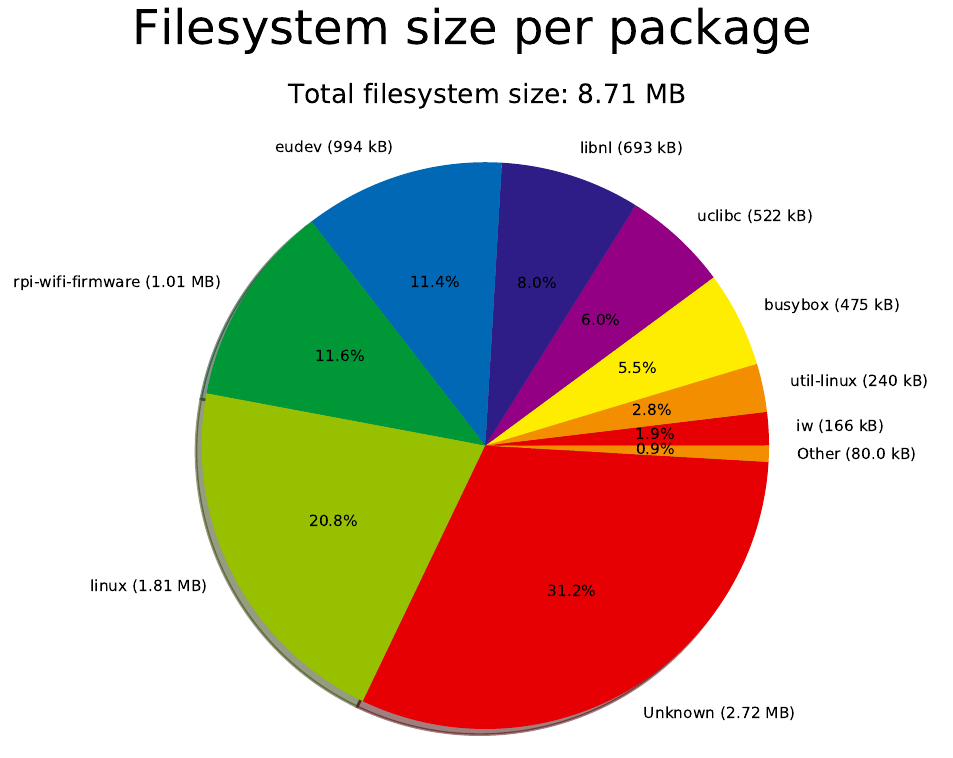
\includegraphics[width=0.7\textwidth]{size.png}
\end{center}

\end{document}